

\chapter{Conclusions}
\epigraphfontsize{\small\itshape}
\setlength\epigraphwidth{8cm}
\setlength\epigraphrule{0pt}

\epigraphfontsize{\small\itshape}
\epigraph{There always remain in the abyss of things slumbering, parts
which have yet to be awakened.}{Gottfried Wilhelm von Leibniz 1697}


This chapter summarizes the thesis, discusses its findings and contributions,
 points out limitations of the current work, and also outlines directions for future research. 

\section{Summary}
In this thesis, a parallel version of the new numerical SCIARA-fv3\cite{Spataro2010} model was implemented
using different GPGPU strategies,
specifically, by adopting the NVIDIA Compute Unified Device Architecture
(CUDA)\cite{NvidiaprogGuide} framework in order to improve the overall execution time.
Following the APOD (see section \ref{sect:APOD}) developing strategy, different
versions were produced, incrementally adding new features and using more
sophisticated CUDA APIs at each developing cycle.
Starting from a naive porting (see section \ref{sect:naiveImplementation}) consisting in a one thread one cell over
the whole cellular space, a LAC version (see section \ref{sect:linearCellAtomic} was developed, that
showed best speedups and occupancy (\(\eta\)) values. Atomic functions (see
sections \ref{sect:atomicImplementation}) were also exploited as
an alternative solution to the non race-condition free flow distribution algorithm
(see section \ref{sect:raceCondAvoiding}).
Tests and numerical analysis were performed in order to understand how to
 maximize the utilization of the available devices and to validate the parallel model implementations. 
Numerical approximation and error propagation were also deeply investigated.

Eventually, a new CUDA C library for CCA were designed, currently in beta-version, permitting an
easy parallel programming of CCA for researchers that are not GPGPU experts to
effortlessly write and execute their CCA models.

\section{Work in progress}
Although the results presented here have demonstrated the effectiveness of the
strategies adopted, parallelization of CCA could be further developed in a
number of ways and some of them are yet on the way to be fully implemented:

\subsection{Multiple Rectangular Bounding Boxes}
RBB as seen in section \ref{sect:RBBOptimization} (at page
\pageref{sect:RBBOptimization}) is a valid solution that permits a good gain in
performance. However, in some situations, it does fit the space of active cells in a
inefficient way. Real occupancy of the device is measured by the ratio
\(\eta=\frac{ACTIVE\_CELLS}{IDLE\_CELLS}\). For example, figure
\ref{fig:activeIdleRatio} shows how \(\eta\) decreases over time.

 Multiple RBB on the same cellular space may lead to higher values of \(\eta\)
 (see figure \ref{fig:MultiRBBExample}) during the execution.
Here, the large single RBB was divided in two smaller RBB, with the property that all
the active cells are inside their boundaries. It's easy to see that the blue
part of the rectangle is composed only by IDLE cells, and no threads are created and
scheduled for execution for those cells.

\begin{figure}
\begin{center}
  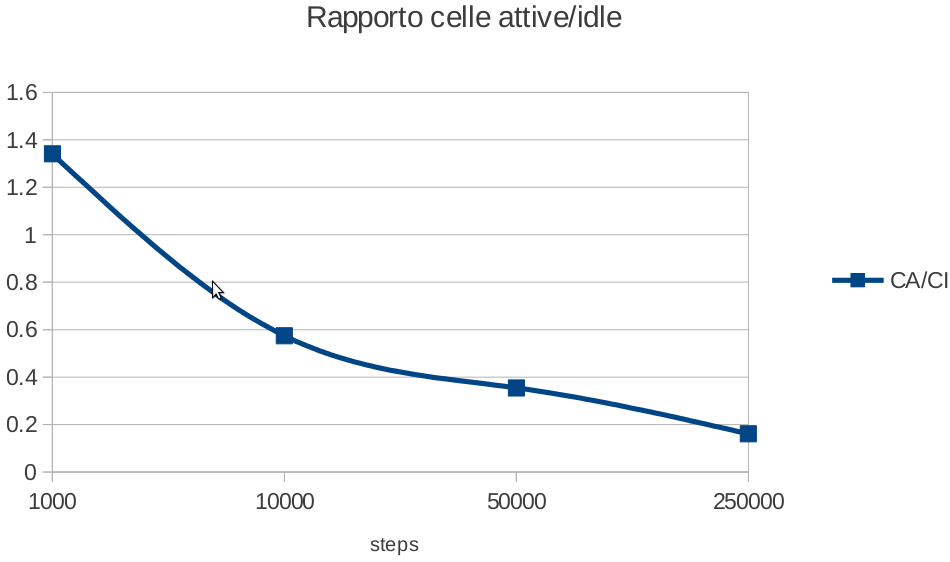
\includegraphics[scale=0.33, trim=0.0cm 0.0cm 0cm 2cm,
  clip=true]{./images/activeIdleRatio}
  \caption{Occupancy ratio during execution of the model on the dataset  :
  \label{fig:activeIdleRatio}
  mount Etna.
  }
\end{center}
\end{figure}


\subsubsection{RBBs positioning and dimensioning}
One of the greater problem in addressing this kind of cellular space management
is to choose how many RBBs have to be utilized and the position of each of them
in order to minimize the number of idle cells. This implies an obvious overhead
due to extra time spent in optimizing their position.
A preliminary adopted solution is to test position of each RBB at different
offsets from the beginning of the cellular space, and choose the combination that guarantees
the minimum number of IDLE cells.
 Another problem can arise from the fact that a
cell may be activated at the same step from two cells belonging to two different
RBB, with the consequence of determining which RBB should take responsibility of the newly activated cell.

\(\eta\) was monitored utilizing up to 4 RBB at the same time, and good results
has appeared (see figure \ref{fig:RBBcomparision}).  



\begin{figure}
\begin{center}
  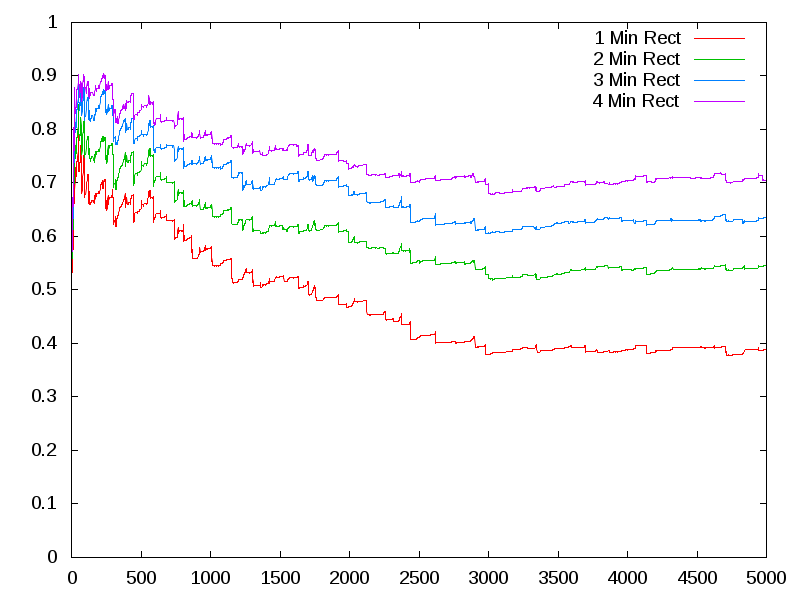
\includegraphics[scale=0.42]{./images/RBBcomparision}
  \caption{Active and Idle cell ratio is
  monitored at each step utilizing up to 4 RBB on the same cellular space.}
  \label{fig:RBBcomparision}
\end{center}
\end{figure}


\subsection{General CCA CUDA-GPGPU library (CuCCAl)}
A GPGPU CUDA powered library \textit{``CuCCAl''}, acronym for ``Cuda
complex cellular automata library'', capable of hiding all the complexity behind
the GPU programming is under development\footnote{An alpha version has been already
released.}. The aim of this library is to make life easier to researchers that need
to parallelize on GPU cellular automata. 
The programmer has only to write the elementary processes that compose the
transition function, register substates and set up some parameters (for
example, the number of steps). \footnote{In next versions these operations may be
automated as well, requiring only a configuration file that lists substates and
parameters.}. Memory management is completely behind the scene, letting the
programmer concentrate only on the model he needs to write.

\subsubsection{Usage overview}
 Listing \ref{code:CuCCAlMain} shows an example of usage of the library.
 
 
 \lstset{label={code:CuCCAlMain},caption={Example of Cuccal usage},
 style=codeStyleC }
\begin{lstlisting}
	int main() {
		/*--------START CONFIGURATION AND INITIALIZATION PHASE--------*/
	
		CA.setInitialParameters(2,2);
		CA.initialize();
	
		CA.addSubstate(Q,BOOL);
		CA.addSubstate(Q_NEW,BOOL);
		
		CA.registerElementaryProcess(gpuEvolve);
		CA.registerElementaryProcess(copyBoard);
		CA.registerStopCondictionCallback(stopCondition);
	
		CA.setBlockDimY(16);
		CA.setBlockdimX(16);
	
		if(CA.loadSubstate(Q,"./data/GOL/initialConfiguration.sst")==ERROR_OPENING_FILE){
			printDebug("ERROR opening file");
			return -1;
		}
	
		CA.initializeGPUAutomata();
	
		/*--------END CONFIGURATION AND INITIALIZATION PHASE--------*/
		CA.globalTransitionFunction();
		CA.copyBuffersFromGPU();
		CA.cleanUpGPUAutomata();
	
		CA.cleanup();
		printf("\nElapsed Time = %.5f \nEND",CA.elapsedTime);
		
		return 0;
	}	
\end{lstlisting} 

The transition function and name of substates have to be specified in a different
file, using a minimal set of CUDA C instructions. \footnote{Programmer has
only to know how the blocks are organized and threads labeled.}
Listing \ref{code:CuCCAlGolDefinition} shows an example of the famous Game of Life Cellular Automaton (see
section \ref{sect:GOL} at \pageref{sect:GOL}) implemented utilizing CuCCAl.


 \lstset{label={code:CuCCAlGolDefinition},caption={Definition of GOL using
 Cuccal library.}, style=codeStyleCUDA }
\begin{lstlisting}
	#include "config.h"
	#include "CA.cuh"
	extern CA CA;
	
	__global__ void gpuEvolve(CA_GPU* d_CA){
		unsigned int col=(threadIdx.x+blockIdx.x*blockDim.x);
		unsigned int row=(threadIdx.y+blockIdx.y*blockDim.y);
		unsigned int totRows=d_CA->scalars->rows;
		unsigned int totCols=d_CA->scalars->cols;
		if(row<totRows && col<totCols){
			short unsigned int count=0;
			unsigned int linNeighIdx=0;
			bool alive=d_CA->getSubstateValue_BOOL(Q,row,col);
			for (int neigh = 1; neigh < 9; neigh++) {
				linNeighIdx=d_CA->getNeighborIndex_MOORE_Toroidal(row,col,neigh,totRows,totCols);
				if(d_CA->getSubstateValue_BOOL(Q,linNeighIdx)==true){
					count++;
				}
			}
			alive=((!alive && count==3) || (alive && ( count==2 || count==3))) ? true : false;
			d_CA->setSubstateValue_BOOL(Q_NEW,row,col,alive);
		}
	}
	void __global__ copyBoard(CA_GPU* d_CA){
		int col=(threadIdx.x+blockIdx.x*blockDim.x);
		int row=(threadIdx.y+blockIdx.y*blockDim.y);
		if(row<d_CA->scalars->rows && col<d_CA->scalars->cols){
			d_CA->setSubstateValue_BOOL(Q,row,col,d_CA->getSubstateValue_BOOL(Q_NEW,row,col));
		}
	}
	//true means --> STOP THE AUTOMATA
	bool stopCondition(){
		if(CA.getSteps()>100){
			return true;
		}
		return false;
	}
	
\end{lstlisting} 
Substate values can be read and written using the set of get and set APIs (see
line 37 in listing \ref{code:CuCCAlMain}).

   \begin{figure}
\begin{center}
  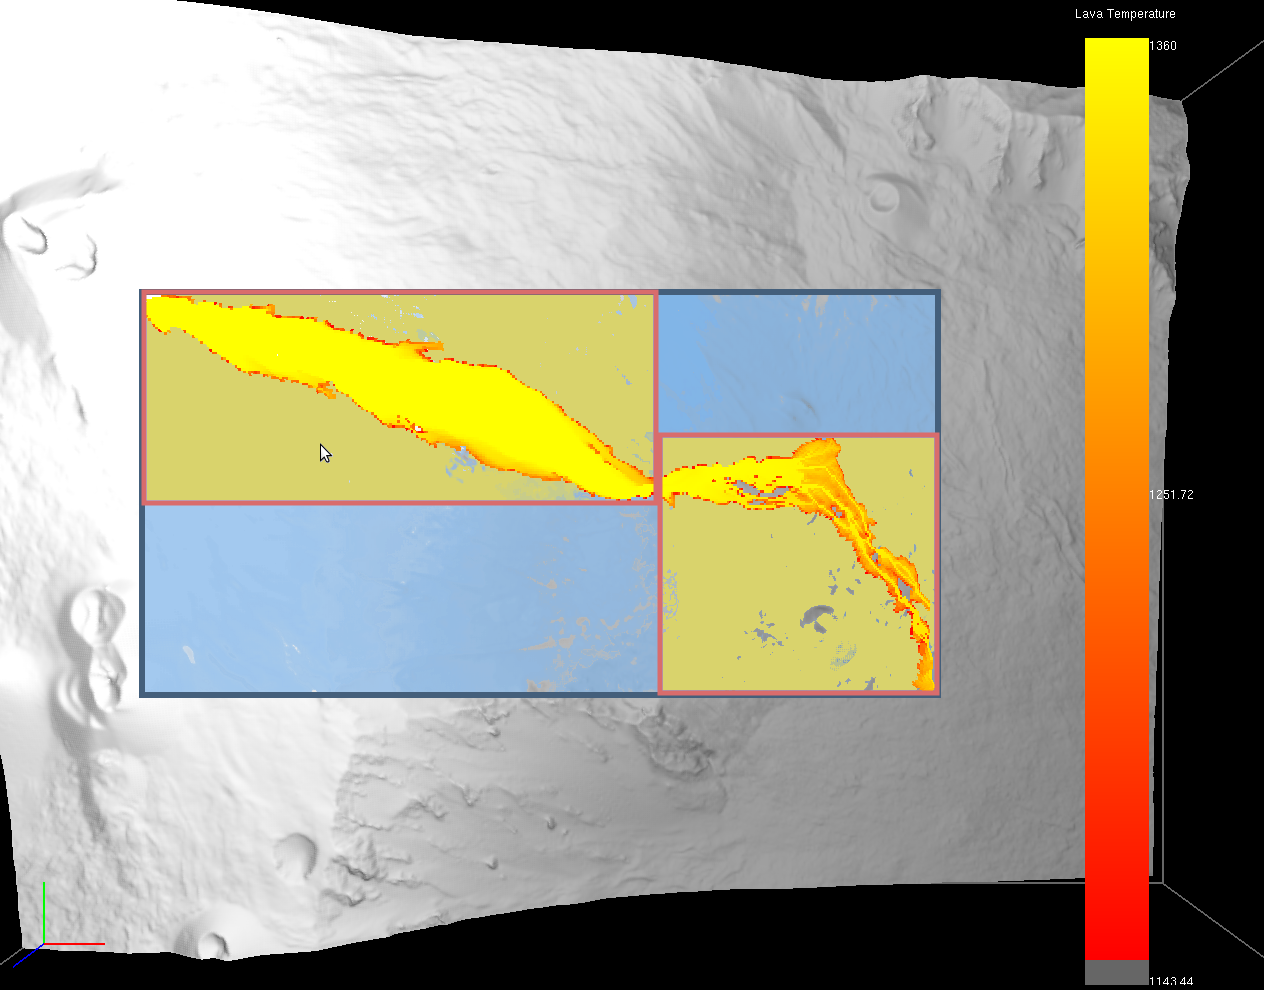
\includegraphics[scale=0.35]{./images/MultiRBBExample}
  \caption[2-RBB cellular space partitioning example]{An example of 2-RBB space
  partitioning.}
  \label{fig:MultiRBBExample}
\end{center}
\end{figure}

\subsubsection{2D GPU Dynamic substate management}
One of the biggest problems in implementing this kind of library is that the number
and datatype of substates are unknown a priori, and hence, the library has to be
powerful enough to dynamically allocate a number of substates that are 1D arrays.
As known, the problem comes from the fact that CUDA disallows usage of 2D matrices and thus array
of pointers cannot be allocated on the GPU. 
The solution consists in allocating and initializing a CPU (and a corresponding copy in GPU) \texttt{d\_subPointer} buffer of GPU arrays.
After this operation,  \texttt{d\_subPointer} is copied back to GPU memory, resulting in 
a C-like dynamic 2D matrix on GPU (see listing \ref{code:CuCCAl2DMatrix}) .

\lstset{label={code:CuCCAl2DMatrix},caption={Double Precision
             atomic operation.}, style=codeStyleCUDA }           
\begin{lstlisting}
	\\GPU matrix
	CUDA_CHECK_RETURN(cudaMalloc((void**)&d_CA_TOCOPY->d_substates,sizeof(void*)*substates_size));
	\\CPU matrix	
	d_subPointer = (void**)malloc(sizeof(void*)*substates_size);
		for(int i=0;i<substates_size;i++){
			d_subPointer[i]=allocateGPUBuffer(d_subPointer[i],(TYPE)substateTypes[i]);
			//legal operation d_subPointer is allocated on GPU
			copyBufferToGPU(d_subPointer[i],substates[i],(TYPE)substateTypes[i]);
			}
			//copy CPUmatrix of GPU pointer  pointers to GPU matrix
		CUDA_CHECK_RETURN(cudaMemcpy(d_CA_TOCOPY->d_substates,d_subPointer,sizeof(void*)*substates_size,cudaMemcpyHostToDevice));
\end{lstlisting} 
 
 
\newpage

\subsection{Publications}

Results of this work have been published in the proceedings of two International
Conferences, namely in the 2014 Parallel, Distributed and Network-Based
Processing (PDP) and the \(9^{th}\) Workshop on Artificial Life and Evolutionary
Computation (Wivace 2014), and submitted to the ISI International Journal of
High Performance and Applications:
  
  \begin{enumerate}
    \item Spataro D., D'Ambrosio D., Filippone G., Spataro W., \textbf{Implementation of the SCIARA-fv3
    parallel numerical model for lava flow simulation by different GPGPU strategies} \emph{International Journal of High Performance and Applications}, submitted.
		\item Spataro W., D'Ambrosio D., Filippone G.,Spataro D., G.
    Iovine, D. Marocco, \textbf{Lava flow modeling by the SCIARA-fv3
    parallel numerical model}, \emph{Proceedings of The 2014 International
    Conference on Parallel, Distributed and Network-Based Processing (PDP)}, Turin, Italy, Feb. 12-14,
    2014.
    \item G. Filippone, R. Parise, D. Spataro,
	D. D’Ambrosio, R. Rongo, and W. Spataro, \textbf{Evolutionary
	applications to Cellular Automata models for volcano risk mitigation},
	\emph{Proceedings of The 2014 International Conference on Workshop on Artificial Life and
	Evolutionary Computation (WIVACE)}, May 14-15 2014, Vietri sul Mare, Salerno,
	Italy.
   
  \end{enumerate}
  
